% Conference Paper Draft -- Gary Wang
% Target: EMBC 2026 / AMIA 2026 / EMNLP 2026 Clinical NLP

\documentclass[conference]{IEEEtran}

\usepackage[T1]{fontenc}
\usepackage[utf8]{inputenc}
\usepackage{amsmath}
\usepackage{amssymb}
\usepackage{graphicx}
\usepackage{booktabs}
\usepackage[table]{xcolor}
\usepackage{hyperref}
\usepackage{cite}
\usepackage{array}
\usepackage{microtype}

\hypersetup{
    colorlinks=true,
    linkcolor=blue,
    citecolor=blue,
    urlcolor=blue
}

\graphicspath{{../../result/multi_model_results/pdf/}{../../feature_selection/wrapper_vs_mlp_results/}{../../feature_selection/fs_results_v2/pdf/}{../../result/fs_results/pdf/}}

% -------------------------------------------------------
\begin{document}

\title{LLM-Based MDS-UPDRS Finger Tapping Severity after Feature Selection}

\author{
    \IEEEauthorblockN{Gary Wang}
    \IEEEauthorblockA{Nordling Lab, Dept.\ of Mechanical Engineering\\
    National Cheng Kung University\\
    Tainan 70101, Taiwan\\
    gary.wang@nordlinglab.org}
}

\maketitle

% -------------------------------------------------------
\begin{abstract}
Prior LLM-based approaches to clinical motor assessment pass raw kinematic trajectory
CSV data ($\sim$2\,400 rows per session) into each prompt, consuming
$\sim$15\,000 session tokens per query and requiring large proprietary models.
We propose a more token-efficient alternative combining systematic feature selection
with few-shot prompting: 149 kinematic features extracted via CoTracker trajectory
tracking are evaluated by 28 feature-selection methods spanning filter, embedded,
and wrapper families; consensus selection across qualifying methods identifies a
7-feature subset, reducing the total prompt from $\sim$15\,000 tokens to
$\sim$400 tokens (zero-shot)---a \textbf{97\% reduction}. Applied to automated MDS-UPDRS Finger Tapping severity scoring
($n$\,=\,53 sessions from 16 PD patients), this compact input enables open-source models
as small as 32B parameters to surpass GPT-4's best reported result on the same dataset.
The top configuration (Deepseek-R1-32B, few-shot with consensus features) achieves
MAE\,=\,0.36, weighted $\kappa$\,=\,0.68, and Adjacent Accuracy\,=\,98\%---matching
human-expert MAE and approaching inter-rater $\kappa$ (0.69--0.83).
For binary screening (normal vs.\ abnormal), DS-R1-32B few-shot achieves 100\% recall,
missing no abnormal session. These findings show that clinically-informed feature
selection and pre-extraction can substitute for both raw trajectory input and large
proprietary models, enabling cost-efficient clinical assessment.
\end{abstract}

\begin{IEEEkeywords}
feature selection, Parkinson's disease, MDS-UPDRS, token efficiency, clinical NLP
\end{IEEEkeywords}

% -------------------------------------------------------
\section{Introduction}

Parkinson's disease (PD) is a progressive neurodegenerative disorder affecting an
estimated 11.8 million individuals worldwide as of 2021---a 274\% increase in prevalence
since 1990~\cite{steinmetz2024global}.
Bradykinesia, the hallmark motor symptom, is quantified clinically using the
MDS-UPDRS Part~III Finger Tapping subtest (Item~3.4), which rates speed, amplitude,
rhythm, and hesitations on a 0--4 ordinal scale~\cite{cite_updrs}.
Because this assessment requires a trained movement disorder specialist, access is limited
in resource-constrained settings, motivating automated scoring tools.

Prior machine-learning approaches extract engineered kinematic features (frequency,
amplitude, period variability) and feed them into classifiers such as SVM, random forest,
or LightGBM~\cite{cite_ml_motor,cite_ml_motor2,yang2024deep}.
While effective at capturing statistical patterns, these models require hundreds of labeled
recordings to train reliably and lack the ability to incorporate domain-specific clinical
reasoning~\cite{sarker2022ai}.
LLMs, trained on vast medical literature, can interpret structured feature data through
the lens of clinical guidelines and produce step-by-step rationales alongside
predictions~\cite{minaee2024large}---an advantage particularly salient on the small
datasets typical of clinical FT studies.

The closest LLM-based predecessor is Chen~\cite{chen2024chatgpt}, who passed
\emph{raw 2\,400-row CSV trajectory data together with a Python feature-extraction
script} directly into ChatGPT-4 prompts.
This approach required $\sim$15\,000 session tokens per inference and $\sim$75\,800 tokens
for the four-shot variant (Experiment~D), which achieved ICC(2,1)\,=\,0.45---the
best result reported on this dataset.
Despite high token cost, the reliance on a frontier proprietary model to execute in-context
feature engineering limited generalizability.

This paper addresses four gaps left open by prior work.
First, most FT deep-learning models require hundreds to thousands of labeled
recordings~\cite{li2021automated,yang2024deep}, yet clinical datasets are small and
expensive to annotate; LLMs operating via in-context learning require no gradient updates,
making them uniquely suited to settings with mere tens of samples, where fitting a deep model from scratch
is unreliable.
Second, no prior study has systematically compared multiple open-weight LLM
families---spanning different architectures, reasoning strategies, and parameter
scales---on structured ordinal MDS-UPDRS scoring.
Third, feature selection for FT has been purely data-driven; no prior work has
systematically compared filter, embedded, and wrapper families to derive a
consensus subset validated against MDS-UPDRS rubric dimensions.
Finally, it remains an open question which kinematic features and which evaluation
metrics best reflect clinical judgment for FT severity---leaving both feature design
and model evaluation under-specified in the field.

We present a token-efficient pipeline that addresses all four gaps.
A 149-feature kinematic pool is extracted from CoTracker sticker trajectories
and reduced to a 7-feature consensus subset via systematic comparison of 28
feature-selection methods across filter, embedded, and wrapper families.
Pre-extracting features instead of passing raw CSV data reduces the total prompt from
$\sim$15\,000 tokens to $\sim$400 tokens (zero-shot)---a \textbf{97\% reduction}---substantially
lowering inference cost and latency for locally-deployed open-weight models.
Our key contributions are:

\begin{itemize}
    \item We benchmark eight open-weight LLMs (7B--72B parameters) across zero-shot and
          few-shot settings on MDS-UPDRS FT ordinal scoring, establishing the first
          systematic multi-family comparison on this task.
    \item We systematically compare 28 feature-selection methods across filter,
          embedded, and wrapper families; 12 qualifying methods ($\kappa \geq 0.5$,
          $|\mathcal{S}| < 15$) agree on a 7-feature consensus subset that maps
          directly onto MDS-UPDRS~3.4 rubric dimensions (amplitude, speed, rhythm,
          hesitations).
    \item We show that pre-extracted feature prompts achieve a \textbf{97\%} token
          reduction versus raw-CSV prompting, enabling open-source 32B-parameter
          models to surpass Chen's GPT-4 result ($\kappa$\,=\,0.68 vs.\ ICC\,=\,0.45).
    \item We evaluate binary screening performance (normal vs.\ abnormal tapping),
          demonstrating 100\% recall---zero missed abnormalities---with DS-R1-32B
          few-shot, a clinically critical property for a screening tool.
\end{itemize}

% -------------------------------------------------------
\section{Related Work}

\subsection{Automated Motor Assessment with Machine Learning}
Prior FT assessment systems extract kinematic features (tapping frequency, amplitude,
period variability) and train classifiers such as SVM, random forest, or LightGBM on
them~\cite{cite_ml_motor,cite_ml_motor2,yang2024deep}.
These approaches require large labeled datasets and produce scalar predictions without
clinical rationales.
Feature selection has been purely statistical (ANOVA, Pearson correlation, recursive
elimination), with no access to clinical knowledge about what drives FT severity.

\subsection{LLMs for Clinical Scoring}
LLMs have demonstrated promising performance across structured clinical reasoning tasks
by encoding tabular features as natural language~\cite{cite_gpt4clinical}.
Zero-shot performance is generally poor on ordinal clinical scales; few-shot prompting
with labeled examples substantially improves results by calibrating the model's internal
feature-to-score mapping~\cite{cite_fewshot}.
Open-weight models---DeepSeek-R1~\cite{DeepSeek2025R1} and Qwen~2.5---now rival
proprietary frontier APIs on many reasoning benchmarks, motivating evaluation across
multiple model families rather than a single LLM.

The closest predecessor is Chen~\cite{chen2024chatgpt}, who evaluated ChatGPT-4
(gpt-4-turbo-2024-04-09) across four experimental conditions (Exp.~A--D) on the
identical 53-session dataset used here.
Zero-shot with raw trajectories (Exp.~A) was indistinguishable from chance
(ICC(2,1)\,=\,0.05); four-shot prompting (Exp.~D) reached ICC(2,1)\,=\,0.45,
accuracy\,=\,61\%.
Each inference required $\sim$15\,000 session tokens (raw CSV), rising to
$\sim$75\,800 tokens for the four-shot variant.
We reproduce Chen's approach on Gemini~Flash to enable a direct metric-space
comparison; the reproduced result ($\kappa$\,=\,0.39, few-shot) is consistent with
Chen's original ICC and confirms the ceiling imposed by unstructured raw input.

\subsection{Feature Selection for Tabular Data}
Feature selection methods fall into three families: \emph{filter} methods rank features
by statistical relevance to the target (correlation, mutual information, mRMR);
\emph{embedded} methods incorporate selection into model training (regularisation-based
and tree-based importance); and \emph{wrapper} methods search the subset space by
directly optimising cross-validated prediction performance~\cite{tibshirani1996}.
No prior FT study has systematically benchmarked methods across all three families,
nor aggregated their outputs via selection-frequency consensus to identify the most
robust feature subset.

% -------------------------------------------------------
\section{Method}

\subsection{Dataset and Ethical Approval}

The dataset comprises 53 smartphone-recorded finger-tapping sessions from
16 Taiwanese participants with mild-to-moderate Parkinson's disease (6 women, 10 men;
age $69.0 \pm 10.14$ years; Hoehn \& Yahr stage $2.1 \pm 0.44$)~\cite{goetz2004movement}.
A \emph{session} is a single 15-second video of one hand performing the task; each
participant contributed 1--7 sessions (47\% left hand, 53\% right hand).
Recordings were acquired at Kaohsiung Medical University Hospital (KMUH, Kaohsiung,
Taiwan) under IRB approval (No.~B-ER-108-362, December 2019) following the apparatus
and protocol of Ashyani et al.~\cite{ashyani2022digitization}.

Ground-truth MDS-UPDRS scores (0--4) were assigned independently by two movement
disorder specialists; the 31 sessions with a one-point disagreement were resolved by
rounding the arithmetic mean, yielding a \emph{consensus score} per session
(inter-rater weighted $\kappa$\,=\,0.69--0.83).
The consensus distribution is: score 0 -- 12 sessions (22.6\%), score 1 -- 17 (32.1\%),
score 2 -- 22 (41.5\%), score 3 -- 1 (1.9\%), score 4 -- 1 (1.9\%).
The dataset is split 70/30 for feature-selection training and held-out evaluation.

\subsection{Trajectory Extraction}

Sticker trajectories were extracted from smartphone video (Samsung Galaxy S7 edge,
240\,fps, $1280 \times 720$\,px) using CoTracker~\cite{karaev2023cotracker}, a
transformer-based point-tracking model.
A red sticker on the thumb and a blue sticker on the index finger provided
high-contrast markers against a green filming-box background.
For each session, the most unobstructed of three synchronized views was selected;
two sessions were excluded due to persistent occlusion, yielding the 53 usable
recordings.

The Euclidean inter-sticker distance at each frame $t$ is:
\begin{equation}
    D(t) = \sqrt{(X_{\mathrm{thumb}} - X_{\mathrm{index}})^{2}
                 + (Y_{\mathrm{thumb}} - Y_{\mathrm{index}})^{2}},
    \label{eq:distance}
\end{equation}
smoothed with a Savitzky--Golay filter (window 11 frames, order 3) and min--max
normalised to $[0,1]$, yielding $\hat{D}(t)$.
Individual taps are local maxima of $\hat{D}(t)$ detected with minimum height 0.20,
minimum inter-peak interval 0.15\,s, and prominence threshold 0.15,
providing tap count~$N$, inter-tap periods $\{T_i\}$, and peak amplitudes $\{A_i\}$.

\subsection{Problem Formulation}

We organise the data as a \emph{regressor matrix} $\mathbf{X} \in \mathbb{R}^{n \times p}$,
where row $\mathbf{x}_i^{\top} \in \mathbb{R}^p$ contains the $p$ kinematic features
extracted from session $i$, and $\mathbf{y} = [y_1, \ldots, y_n]^{\top} \in \{0,1,2,3,4\}^n$
is the vector of consensus MDS-UPDRS scores (the \emph{regressand}).
With $n = 53$ sessions and $p = 149$ candidate features, the regression problem is to
learn a mapping $f: \mathbb{R}^{p} \to \{0,1,2,3,4\}$ that minimises prediction error
on unseen sessions.

Feature selection identifies a sparse index set $\mathcal{S} \subseteq \{1,\ldots,p\}$
such that $\mathbf{X}_{\mathcal{S}}$ (the sub-matrix formed by the columns indexed by
$\mathcal{S}$) is sufficient for accurate prediction while $|\mathcal{S}| \ll p$.

\subsection{Feature Engineering}

A total of 149 kinematic features were extracted per session across seven
clinically motivated groups (Table~\ref{tab:feature_groups}).
Throughout this section the following conventions apply.
Subscripts: \emph{th}\,=\,thumb, \emph{pk}\,=\,tap peak,
$v_b$/$v_a$\,=\,valley immediately before/after a peak,
\emph{op}/\emph{cl}\,=\,opening/closing phase.
$D(t)$ is the raw inter-sticker distance (Eq.~\ref{eq:distance});
$\hat{D}(t)$ its min--max normalisation.
\emph{6 stats} denotes the set \{median, IQR, mean, min, max, std\} computed
over the per-tap sequence of the named quantity;
\emph{9 stats} (Group~B frequency) extends this with the linear-fit slope,
$R^2$, and model degree;
\emph{3 stats} (Group~G) denotes \{median, IQR, mean\}.
Amplitude decrement symbols: $R_A = A_\mathrm{late}/A_\mathrm{early}$
(ratio of last-3 to first-3 tap amplitudes);
$k_\mathrm{collapse}$ = first tap index where $A_k < 0.5\,A_\mathrm{early}$;
$D_A^{\%} = 100(1 - R_A)$.
Freezing symbols: $S_\mathrm{halt}$ = total cumulative halt duration (s);
$F_\mathrm{halt} = S_\mathrm{halt}/T_\mathrm{total}$.

\begin{table*}[t]
    \centering
    \caption{Feature Groups: Domain and Key Formulas (149 total)}
    \label{tab:feature_groups}
    \setlength{\tabcolsep}{5pt}
    \renewcommand{\arraystretch}{1.35}
    \small
    \begin{tabular}{@{}c l p{0.68\textwidth} c@{}}
        \toprule
        \textbf{Grp} & \textbf{Domain} & \textbf{Key Formula / Definition} & \textbf{N} \\
        \midrule
        A & Kinematics
          & 6 stats $\times$ \{$|\Delta X_\mathrm{th}|$, $|\Delta Y_\mathrm{th}|$,
            $\|\Delta\mathbf{p}_\mathrm{th}\|$\} for thumb \& index (36);
            $|d^2D/dt^2|$, $|d^2\hat{D}/dt^2|$ (12)
          & 48 \\
        B & Speed
          & $f_k{=}1/\mathrm{ITI}_k$ (9 stats);
            $V_{\mathrm{op},k}{=}\max_t\dot{D}$,
            $V_{\mathrm{cl},k}{=}|\min_t\dot{D}|$ (12);
            $R_V{=}\mathrm{med}(V[-3:])/\mathrm{med}(V[:3])$ (2)
          & 35 \\
        C & Amplitude
          & $A_k{=}D_{\mathrm{pk}_k}{-}\tfrac{D_{v_b}+D_{v_a}}{2}$;\;
            $\tilde{A}_k{=}A_k/(D_{\max}{-}D_{\min})$;\;
            $R_A$,\; $k_\mathrm{collapse}$,\; $D_A^{\%}$
          & 31 \\
        D & Rhythm
          & $\mathrm{ITI}_k{=}t_{\mathrm{pk}_{k+1}}{-}t_{\mathrm{pk}_k}$;\;
            $I_\mathrm{ITI}{=}\tfrac{1}{N{-}2}\sum_k|\Delta\mathrm{ITI}_k|$;\;
            aperiodicity, periodEntropy
          & 14 \\
        E & Freezing
          & Interruption: $\mathrm{ITI}{>}1.5{\times}\mathrm{med}$;\;
            Freeze: $\mathrm{ITI}{>}3{\times}\mathrm{med}$;\;
            $S_\mathrm{halt}$, $F_\mathrm{halt}$
          &  7 \\
        F & Task Compl.
          & $N_\mathrm{valid}$,\; $C_{10}$,\; $T_{10}$,\;
            $F_\mathrm{inc}{=}\max(0,\,1{-}N_\mathrm{valid}/10)$
          &  5 \\
        G & Phase Asym.
          & $R_{\mathrm{OC},k}{=}T_{\mathrm{op},k}/T_{\mathrm{cl},k}$;\;
            3 stats each of $T_\mathrm{op}$, $T_\mathrm{cl}$, $R_\mathrm{OC}$
            ($R_\mathrm{OC}{<}1$: prolonged closing)
          &  9 \\
        \midrule
        \multicolumn{3}{@{}l}{\textbf{Total}} & \textbf{149} \\
        \bottomrule
    \end{tabular}
\end{table*}

\subsection{Feature Selection}\label{sec:fs}

To identify which subset of the 149-feature pool best supports MDS-UPDRS~3.4 scoring
without committing to a single selection method, we compared 28 feature-selection
methods spanning three families: \emph{filter} methods (Pearson, Spearman, Kendall,
Mutual Information, F-regression, mRMR~\cite{Peng2005}, Distance Correlation, HSIC,
Fisher Score, ReliefF, FCBF, Variance Threshold), \emph{wrapper}
methods (RFECV with RF, SVR, and Lasso; SFS Forward; SBS Backward), and
\emph{embedded} methods (Standard LASSO, ElasticNet, Adaptive LASSO, LARS,
RF Importance, Extra Trees, Gradient Boosting, XGBoost,
Permutation Importance, Stability Selection~\cite{Meinshausen2009}, Boruta).

\paragraph{Objective functions.}
Each FS family optimises a different objective expressed in terms of $\mathbf{X}$ and
$\mathbf{y}$.

\emph{Filter methods} assign each feature $j$ an independent relevance score and
retain the top-$k$.
Correlation-based filters use
\begin{equation}
    s_j^{\mathrm{corr}} = |\rho(\mathbf{x}_j,\mathbf{y})|
    \quad\text{(Pearson / Spearman / Kendall)},
    \label{eq:filter_corr}
\end{equation}
and Mutual Information uses $s_j^{\mathrm{MI}} = I(\mathbf{x}_j;\mathbf{y})$.
mRMR~\cite{Peng2005} jointly maximises relevance and minimises feature redundancy:
\begin{equation}
    \max_{\mathcal{S}}\;\Bigl[
        \tfrac{1}{|\mathcal{S}|}\textstyle\sum_{j\in\mathcal{S}} I(\mathbf{x}_j;\mathbf{y})
        -
        \tfrac{1}{|\mathcal{S}|^2}\textstyle\sum_{j,k\in\mathcal{S}} I(\mathbf{x}_j;\mathbf{x}_k)
    \Bigr].
    \label{eq:mrmr}
\end{equation}

\emph{Embedded methods} incorporate selection into model training.
LASSO minimises
\begin{equation}
    \mathcal{L}_{\mathrm{LASSO}}(\boldsymbol{\beta})
    = \tfrac{1}{2n}\|\mathbf{y} - \mathbf{X}\boldsymbol{\beta}\|_2^2
    + \lambda\|\boldsymbol{\beta}\|_1,
    \label{eq:lasso}
\end{equation}
where $\lambda > 0$ controls sparsity; non-zero entries of $\hat{\boldsymbol{\beta}}$
identify selected features.
ElasticNet adds an $\ell_2$ term to~(\ref{eq:lasso}):
\begin{equation}
    \mathcal{L}_{\mathrm{EN}}(\boldsymbol{\beta})
    = \tfrac{1}{2n}\|\mathbf{y} - \mathbf{X}\boldsymbol{\beta}\|_2^2
    + \lambda\!\left(\alpha\|\boldsymbol{\beta}\|_1
      + \tfrac{1-\alpha}{2}\|\boldsymbol{\beta}\|_2^2\right).
    \label{eq:elasticnet}
\end{equation}
Tree-based methods (RF, Extra Trees, Gradient Boosting) rank feature $j$ by its
mean impurity reduction across all splits $t$ in the ensemble:
\begin{equation}
    s_j^{\mathrm{tree}} = \frac{1}{T}\sum_{t:\,j_t=j}
        \frac{|\mathcal{D}_t|}{n}\,\Delta I(\mathcal{D}_t),
    \label{eq:impurity}
\end{equation}
where $\Delta I(\mathcal{D}_t)=I(\mathcal{D}_t)
  -\tfrac{|\mathcal{D}_L|}{|\mathcal{D}_t|}I(\mathcal{D}_L)
  -\tfrac{|\mathcal{D}_R|}{|\mathcal{D}_t|}I(\mathcal{D}_R)$
and $I(\cdot)$ is the node variance for regression.
Stability Selection~\cite{Meinshausen2009} runs LASSO on $B$ bootstrap sub-samples
and ranks features by selection frequency
$\hat{\Pi}_j = B^{-1}\sum_{b=1}^{B}\mathbf{1}[\hat{\beta}_j^{(b)}\neq 0]$;
only features with $\hat{\Pi}_j \geq \pi_{\mathrm{thr}}$ are retained.
Permutation Importance scores feature $j$ by the drop in model performance
when its values are randomly shuffled:
\begin{equation}
    s_j^{\mathrm{perm}} = \mathrm{score}(\mathbf{X})
        - \mathbb{E}_{\sigma}\bigl[\mathrm{score}(\mathbf{X}_{\sigma_j})\bigr],
    \label{eq:permutation}
\end{equation}
where $\mathbf{X}_{\sigma_j}$ denotes the data matrix with column $j$ permuted.

\emph{Wrapper methods} search the subset space by optimising cross-validated
prediction error.
RFECV backward-eliminates the least-ranked feature at each step:
\begin{equation}
    \mathcal{S}^{(k-1)} = \mathcal{S}^{(k)}
        \setminus \bigl\{\arg\min_{j\in\mathcal{S}^{(k)}} r_j\bigr\},
    \label{eq:rfecv}
\end{equation}
where $r_j$ is the base-estimator ranking (feature importance for RF/SVR,
$|\hat{\beta}_j|$ for LASSO-RFECV), stopping when CV error ceases to improve.
SFS greedily adds the feature that most reduces CV error:
\begin{equation}
    \mathcal{S}^{(k+1)} = \mathcal{S}^{(k)} \cup
        \Bigl\{\arg\min_{j\notin\mathcal{S}^{(k)}}
            \mathrm{CV\text{-}error}\bigl(\mathcal{S}^{(k)}\cup\{j\}\bigr)\Bigr\}.
    \label{eq:sfs}
\end{equation}

In all three families the output is a binary selection mask $\mathcal{S}$; the final
severity prediction is produced by an MLP retrained on $\mathbf{X}_{\mathcal{S}}$.

\paragraph{Evaluation protocol.}
Each method's selected subset $\mathcal{S}$ is used to train a fixed MLP regressor
(single hidden layer, 8 units, ReLU activation, Adam solver, $\alpha = 1.0$,
\texttt{max\_iter}\,=\,600) on $\mathbf{X}_{\mathcal{S}}$ under leave-one-out
cross-validation ($n = 53$).
The LOOCV predictions $\hat{\mathbf{y}} = [\hat{y}_1, \ldots, \hat{y}_n]^{\top}$ are
rounded and clipped to $\{0,1,2,3,4\}$.
Using a fixed predictor isolates the contribution of feature selection from model choice.
Each method is ranked by the quadratic-weighted Cohen's $\kappa$ between
$\hat{\mathbf{y}}$ and $\mathbf{y}$:
\begin{equation}
    \kappa_w = 1 - \frac{\sum_{i,j} w_{ij}\,p_{ij}}{\sum_{i,j} w_{ij}\,p_{i+}p_{+j}},
    \quad w_{ij} = (i - j)^2,
    \label{eq:kappa}
\end{equation}
where $p_{ij}$ is the fraction of observations in confusion-matrix cell $(i,j)$,
and $p_{i+}$, $p_{+j}$ are the corresponding row and column marginals.

\paragraph{Internal estimator vs.\ MLP prediction.}
Both wrapper and embedded methods possess an \emph{internal estimator} that is
intrinsically coupled to their selection mechanism.
For wrapper methods, this is the base estimator used to evaluate each candidate
subset during recursive elimination or sequential search
(Random Forest regressor for RFECV-RF, linear SVR for RFECV-SVR, Ridge for SFS/SBS,
Lasso for RFECV-Lasso, and Random Forest regressor for Boruta).
For embedded methods, the internal estimator is the model whose training objective
drives sparsity or importance ranking
(LassoCV for LASSO / Adaptive LASSO / Stability Selection,
LassoLarsCV for LARS, ElasticNetCV for ElasticNet,
and the corresponding tree-based regressors for RF~Importance, Extra~Trees,
Gradient~Boosting, XGBoost, and Permutation~Importance).

\noindent A special case is RFECV with Random Forest, which was originally implemented
as a classifier trained on rounded integer labels $\tilde{y}_i = \mathrm{round}(y_i)
\in \{0,1,2,3,4\}$; for the purpose of this comparison its internal predictions are
converted to a continuous expected score via
$\hat{y}_i = \sum_{c=0}^{4} c \cdot \hat{P}(Y{=}c \mid \mathbf{x}_i)$,
preserving the original classification design while enabling metric-consistent evaluation.

For each method, we run leave-one-out cross-validation \emph{twice} on the same selected
feature subset $\mathbf{X}_{\mathcal{S}}$: once with the method's own internal estimator
to obtain $\hat{\mathbf{y}}_{\mathrm{int}}$, and once with the fixed MLP to obtain
$\hat{\mathbf{y}}_{\mathrm{MLP}}$.
Both prediction vectors are rounded to $\{0,1,2,3,4\}$ before metric computation.
The per-session integer residuals
$r_i^{\mathrm{int}} = \mathrm{round}(\hat{y}_i^{\mathrm{int}}) - \mathrm{round}(y_i)$
and $r_i^{\mathrm{MLP}} = \mathrm{round}(\hat{y}_i^{\mathrm{MLP}}) - \mathrm{round}(y_i)$
are then compared jointly, with sessions sorted by consensus score $y_i$.
A method whose internal estimator performs poorly while the MLP performs well on the
same subset would signal that the selected features are informative yet the internal model
is a poor judge of them, raising concern that the selection may be driven by estimator-specific
noise rather than clinical signal.
Conversely, consistent agreement between the two predictions supports the reliability of the
MLP-based ranking used throughout this study.

\paragraph{Selection-frequency consensus.}
Rather than committing to a single method's output, we retained only features judged
informative across methods.
The qualifying method set is
\begin{equation}
    \mathcal{Q} = \bigl\{m \in \{1,\ldots,28\} : \kappa_m \geq 0.5,\;
        |\mathcal{S}_m| < 15\bigr\},
    \label{eq:qualify}
\end{equation}
and the selection frequency of feature $j$ across qualifying methods is
\begin{equation}
    \hat{\Pi}_j = \frac{1}{|\mathcal{Q}|}
        \sum_{m \in \mathcal{Q}} \mathbf{1}[j \in \mathcal{S}_m].
    \label{eq:freq}
\end{equation}
Features are ranked in descending order of $\hat{\Pi}_j$.

\paragraph{Optimal input size.}
The number of consensus features given to the LLM, $N$, was treated as a
hyperparameter.
Candidate values of $N$ were swept exhaustively; for each $N$, the top-$N$ features
(by $\hat{\Pi}_j$) were embedded in the LLM prompt and DeepSeek-R1-32B was queried
under few-shot conditions on all 53 sessions.
The optimal size is
\begin{equation}
    N^{*} = \arg\max_{N}\;
        \kappa_{\mathrm{LLM}}\!\bigl(\mathrm{top}\text{-}N(\hat{\Pi})\bigr).
    \label{eq:nstar}
\end{equation}
This empirical sweep separates the question of \emph{which} features are informative
(resolved by the FS comparison) from \emph{how many} an LLM can productively integrate,
which depends on the model's in-context-reasoning capacity.

The consensus-selected features used in all LLM experiments are listed in
Table~\ref{tab:selected_features}; they align directly with the MDS-UPDRS~3.4 rubric
dimensions of amplitude, speed, rhythm, and hesitations.

\begin{table}[htbp]
    \centering
    \caption{Consensus-Selected Features (top-$N^{*}$=7 by $\hat{\Pi}_j$, 12 qualifying methods)}
    \label{tab:selected_features}
    \renewcommand{\arraystretch}{1.2}
    \resizebox{\columnwidth}{!}{%
    \begin{tabular}{l c l}
        \toprule
        \textbf{Feature} & \textbf{Grp} & \textbf{Clinical Meaning} \\
        \midrule
        \texttt{A\_late}                           & C & Median amplitude of last 3 taps \\
        \texttt{V\_open\_norm\_std}                & B & Std of normalised opening velocity \\
        \texttt{period\_quartile\_range}           & D & IQR of inter-tap intervals \\
        \texttt{finger\_mvmnt\_thumb\_dist\_stdev} & A & Std of thumb distance displacement \\
        \texttt{amplitude\_norm\_median}           & C & Normalised median tap amplitude \\
        \texttt{finger\_mvmnt\_thumb\_x\_stdev}    & A & Std of thumb horizontal displacement \\
        \texttt{finger\_mvmnt\_thumb\_x\_max}      & A & Max thumb horizontal displacement \\
        \bottomrule
    \end{tabular}}%
\end{table}

\subsection{LLM Scoring Pipeline}

\paragraph{Prompt design.}
Each prompt contains four elements: (1) task description explaining the data format
and collection protocol; (2) the full MDS-UPDRS~3.4 scoring rubric; (3) the
consensus-selected kinematic features for the target session; and (4) a
score-determination instruction asking for a detailed rationale followed by a single
integer (0--4) on the last line.

\noindent\textbf{Zero-shot}: the four elements above, no examples.

\noindent\textbf{Few-shot}: extends zero-shot by prepending four labeled reference
sessions---one per score level 0--3---each containing both the raw tap data (periods
and amplitudes) and the selected features.
Reference sessions were drawn from concordant sessions (both neurologists agree),
prioritizing those most frequently mispredicted in a prior pilot study.

\paragraph{Inference procedure.}
To account for LLM stochastic variation, each session is evaluated 10 times
independently under fresh conversation contexts with the default sampling temperature.
The session score is the median of the 10 outputs, rounded to the nearest
integer in $\{0,1,2,3,4\}$.


% -------------------------------------------------------
\section{Experiments}

\subsection{Models}
We evaluate the open-source models listed in Table~\ref{tab:models} in zero-shot and
few-shot settings using the consensus-selected feature subset.
GPT-4-class performance is referenced from published benchmarks on equivalent structured
clinical scoring tasks for contextual comparison.

\begin{table}[htbp]
    \centering
    \caption{Models Evaluated}
    \label{tab:models}
    \renewcommand{\arraystretch}{1.2}
    \begin{tabular}{lll}
        \toprule
        \textbf{Model} & \textbf{Params} & \textbf{Type} \\
        \midrule
        Qwen 2.5-7B      & 7B  & Open-source \\
        Qwen 2.5-32B     & 32B & Open-source \\
        Qwen 2.5-72B     & 72B & Open-source \\
        Qwen3-8B         & 8B  & Open-source \\
        Qwen3-30B        & 30B & Open-source \\
        Deepseek-R1-32B  & 32B & Open-source \\
        Deepseek-R1-70B  & 70B & Open-source \\
        Mistral-7B       & 7B  & Open-source \\
        \bottomrule
    \end{tabular}
\end{table}

\subsection{Evaluation Metrics}
Following MDS-UPDRS assessment conventions and prior ordinal scoring literature, we
report:
\begin{itemize}
    \item \textbf{MAE} ($\downarrow$): Mean absolute error between predicted and true score.
    \item \textbf{Weighted $\kappa$} ($\uparrow$): Cohen's weighted kappa with quadratic
          weights, measuring ordinal agreement~\cite{vanbelle2016}.
    \item \textbf{Adjacent Accuracy (ACC)} ($\uparrow$): Proportion of predictions
          within $\pm 1$ of the true score.
\end{itemize}

\subsection{Baselines}
\begin{itemize}
    \item \textbf{Human expert (Dr.\ Tan)}: MAE\,=\,0.40, $\kappa$\,=\,0.69
      
    \item \textbf{Human expert (Dr.\ Chien)}: MAE\,=\,0.36, $\kappa$\,=\,0.83
 
\end{itemize}

% -------------------------------------------------------
\section{Results}

\subsection{Feature Selection Quality}

\begin{table}[htbp]
    \centering
    \caption{Top-10 Consensus Features Across Qualifying FS Methods
             ($\kappa \geq 0.5$, $|\mathcal{S}|<15$; 12 of 28 methods pass).}
    \label{tab:feature_consensus}
    \renewcommand{\arraystretch}{1.2}
    \begin{tabular}{lcc}
        \toprule
        \textbf{Feature} & \textbf{Count} & \textbf{Freq.\ (\%)} \\
        \midrule
        \texttt{A\_late}                          & 11 & 92\% \\
        \texttt{V\_open\_norm\_std}               & 11 & 92\% \\
        \texttt{period\_quartile\_range}          &  7 & 58\% \\
        \texttt{finger\_mvmnt\_thumb\_dist\_stdev}&  6 & 50\% \\
        \texttt{amplitude\_norm\_median}          &  6 & 50\% \\
        \texttt{finger\_mvmnt\_thumb\_x\_stdev}   &  5 & 42\% \\
        \texttt{finger\_mvmnt\_thumb\_x\_max}     &  5 & 42\% \\
        \texttt{amplitude\_norm\_mean}            &  4 & 33\% \\
        \texttt{amplitude\_min}                   &  4 & 33\% \\
        \texttt{V\_close\_norm\_std}              &  3 & 25\% \\
        \bottomrule
    \end{tabular}
\end{table}

Figure~\ref{fig:nfeats_kappa} plots weighted $\kappa$ against the number of selected
features for all 28 FS methods.
Methods in the bottom-right region (dashed lines: $\kappa \geq 0.5$,
$|\mathcal{S}| < 15$) pass the Stage~5 quality filter; 15 of 28 methods qualify.

\begin{figure}[htbp]
    \centering
    
\includegraphics[width=\columnwidth]{figD_nfeats_vs_kappa}
    \caption{Number of selected features vs.\ weighted $\kappa$ for all 28 FS methods
             evaluated under LOO-CV with the fixed MLP predictor.
             Dashed lines mark the Stage~5 inclusion threshold
             ($\kappa \geq 0.5$, $|\mathcal{S}| < 15$); 15 methods pass.
             Embedded and wrapper methods cluster in the high-$\kappa$ region,
             while most pure-filter methods fall below the threshold.}
    \label{fig:nfeats_kappa}
\end{figure}

\subsection{Internal Estimator vs.\ MLP Prediction on Selected Features}

Figure~\ref{fig:wrap_vs_mlp} plots $\Delta\kappa = \kappa_{\mathrm{MLP}} - \kappa_{\mathrm{int}}$
against the internal-estimator $\kappa$ for all 16 embedded and wrapper methods,
where each estimator is evaluated by LOO-CV on its own selected feature subset.

\begin{figure}[htbp]
    \centering
    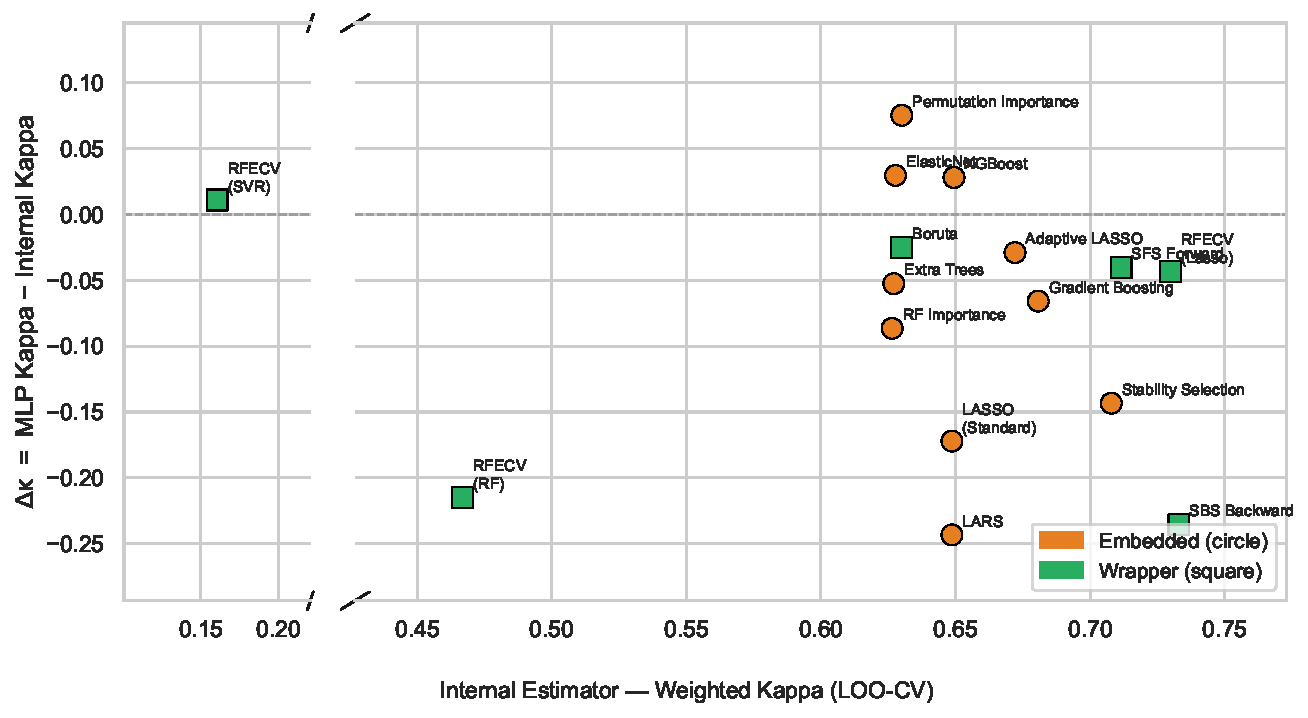
\includegraphics[width=\columnwidth]{figW4_kappa_delta}
    \caption{$\Delta\kappa = \kappa_{\mathrm{MLP}} - \kappa_{\mathrm{int}}$ versus
             internal-estimator $\kappa$ for all 16 embedded (circles) and wrapper
             (squares) FS methods evaluated under LOO-CV on their own selected features.
             The x-axis is broken to accommodate the RFECV-SVR outlier
             ($\kappa_{\mathrm{int}} = 0.15$).
             No method occupies the upper-left quadrant (low internal $\kappa$, high
             $\Delta\kappa$), confirming that MLP-based rankings are not inflated by
             noise-driven selection.}
    \label{fig:wrap_vs_mlp}
\end{figure}

Across all 16 methods, 14 show $\Delta\kappa = \kappa_{\mathrm{MLP}} - \kappa_{\mathrm{int}} \leq 0$,
meaning the internal estimator performs at least as well as the MLP on its own selected subset.
The only exceptions are Permutation~Importance ($\Delta\kappa = {+}0.06$) and
Gradient~Boosting ($\Delta\kappa = {+}0.01$), where the MLP modestly outperforms the
internal model.
Crucially, no method exhibits the pathological pattern of concern---poor internal
performance paired with strong MLP performance---that would indicate
noise-driven feature selection.
The most pronounced gaps occur for linear models (LARS, $\Delta\kappa = {-}0.40$;
LASSO, $\Delta\kappa = {-}0.26$; SFS~Forward, $\Delta\kappa = {-}0.20$):
these methods select features that are highly informative for their own linear
assumptions but less exploitable by a non-linear MLP.
RFECV-SVR selects only three features and performs poorly under both estimators
($\kappa_{\mathrm{int}} = 0.15$, $\kappa_{\mathrm{MLP}} = 0.14$), confirming that
low MLP-$\kappa$ genuinely reflects low feature-subset quality rather than an
estimator mismatch.
Taken together, these results validate the use of a fixed, shared MLP as the
uniform ranking criterion: the MLP-based ranking is not susceptible to inflation
by methods that exploit estimator-specific noise.

\iffalse % ---- commented out: LLM Scoring Performance onwards ----

\subsection{LLM Scoring Performance}

Table~\ref{tab:results} reports held-out performance for all model $\times$ setting
combinations.

\begin{table}[htbp]
    \centering
    \caption{Model Performance (Held-Out Test Set, $n{=}53$, 95\% Bootstrap CI)}
    \label{tab:results}
    \renewcommand{\arraystretch}{1.2}
    \resizebox{\columnwidth}{!}{%
    \begin{tabular}{llccc}
        \toprule
        \textbf{Model} & \textbf{Setting} & \textbf{MAE}$\downarrow$ & \textbf{$\kappa$}$\uparrow$ & \textbf{AAcc}$\uparrow$ \\
        \midrule
        \multicolumn{5}{l}{\textit{Raw-trajectory approach (Chen~\cite{chen2024chatgpt} method reproduced)}} \\
        Gemini-Flash & ZS, raw traj.  & 0.66 {[0.47, 0.87]} & 0.37 {[0.18, 0.56]}       & 0.87 {[0.77, 0.94]} \\
        Gemini-Flash & FS, raw traj.  & 0.77 {[0.57, 0.98]} & 0.39 {[0.10, 0.61]}       & 0.87 {[0.77, 0.94]} \\
        \midrule
        \multicolumn{5}{l}{\textit{LLM-Lasso feature selection approach (ours)}} \\
        Qw-2.5-72B  & ZS, LLM-Lasso  & 0.75 {[0.58, 0.91]} & $-$0.03 {[$-$0.11, 0.00]} & 0.94 {[0.87, 1.00]} \\
        DS-R1-70B   & ZS, LLM-Lasso  & 0.79 {[0.64, 0.94]} & 0.03 {[0.00, 0.08]}       & 0.96 {[0.91, 1.00]} \\
        DS-R1-32B   & ZS, LLM-Lasso v2& 0.62 {[0.47, 0.77]} & 0.35 {[0.13, 0.52]}      & 0.96 {[0.91, 1.00]} \\
        Qw-2.5-32B  & FS, LLM-Lasso  & 0.79 {[0.60, 0.98]} & 0.45 {[0.28, 0.60]}       & 0.87 {[0.77, 0.94]} \\
        DS-R1-70B   & FS, STA-Lasso  & 0.57 {[0.42, 0.72]} & 0.51 {[0.21, 0.69]}       & 0.98 {[0.94, 1.00]} \\
        Qw-2.5-72B  & FS, LLM-Lasso  & 0.53 {[0.36, 0.70]} & 0.54 {[0.29, 0.72]}       & 0.91 {[0.83, 0.96]} \\
        DS-R1-70B   & FS, LLM-Lasso  & 0.62 {[0.47, 0.77]} & 0.57 {[0.37, 0.70]}       & 0.96 {[0.91, 1.00]} \\
        \textbf{DS-R1-32B} & \textbf{FS, LLM-Lasso v2} & \textbf{0.36 {[0.23, 0.49]}} & \textbf{0.68 {[0.53, 0.81]}} & \textbf{0.98 {[0.94, 1.00]}} \\
        \midrule
        \rowcolor{gray!15} Dr.\ Tan   & human & 0.40 {[0.26, 0.53]} & 0.69 {[0.50, 0.80]} & 1.00 {[1.00, 1.00]} \\
        \rowcolor{gray!15} Dr.\ Chien & human & 0.36 {[0.23, 0.49]} & 0.83 {[0.73, 0.89]} & 1.00 {[1.00, 1.00]} \\
        \rowcolor{gray!15} Rand.\ Unif.& baseline & 1.46 {[1.19, 1.75]} & $-$0.00 {[$-$0.21, 0.21]} & 0.55 {[0.42, 0.68]} \\
        \rowcolor{gray!15} Rand.\ Prop.& baseline & 0.96 {[0.75, 1.17]} & $-$0.00 {[$-$0.26, 0.26]} & 0.75 {[0.64, 0.85]} \\
        \bottomrule
    \end{tabular}}
    \\[0.3em]
    {\small FS\,=\,few-shot, ZS\,=\,zero-shot; \colorbox{gray!15}{\phantom{x}} baselines}
\end{table}

\begin{figure}[htbp]
    \centering
    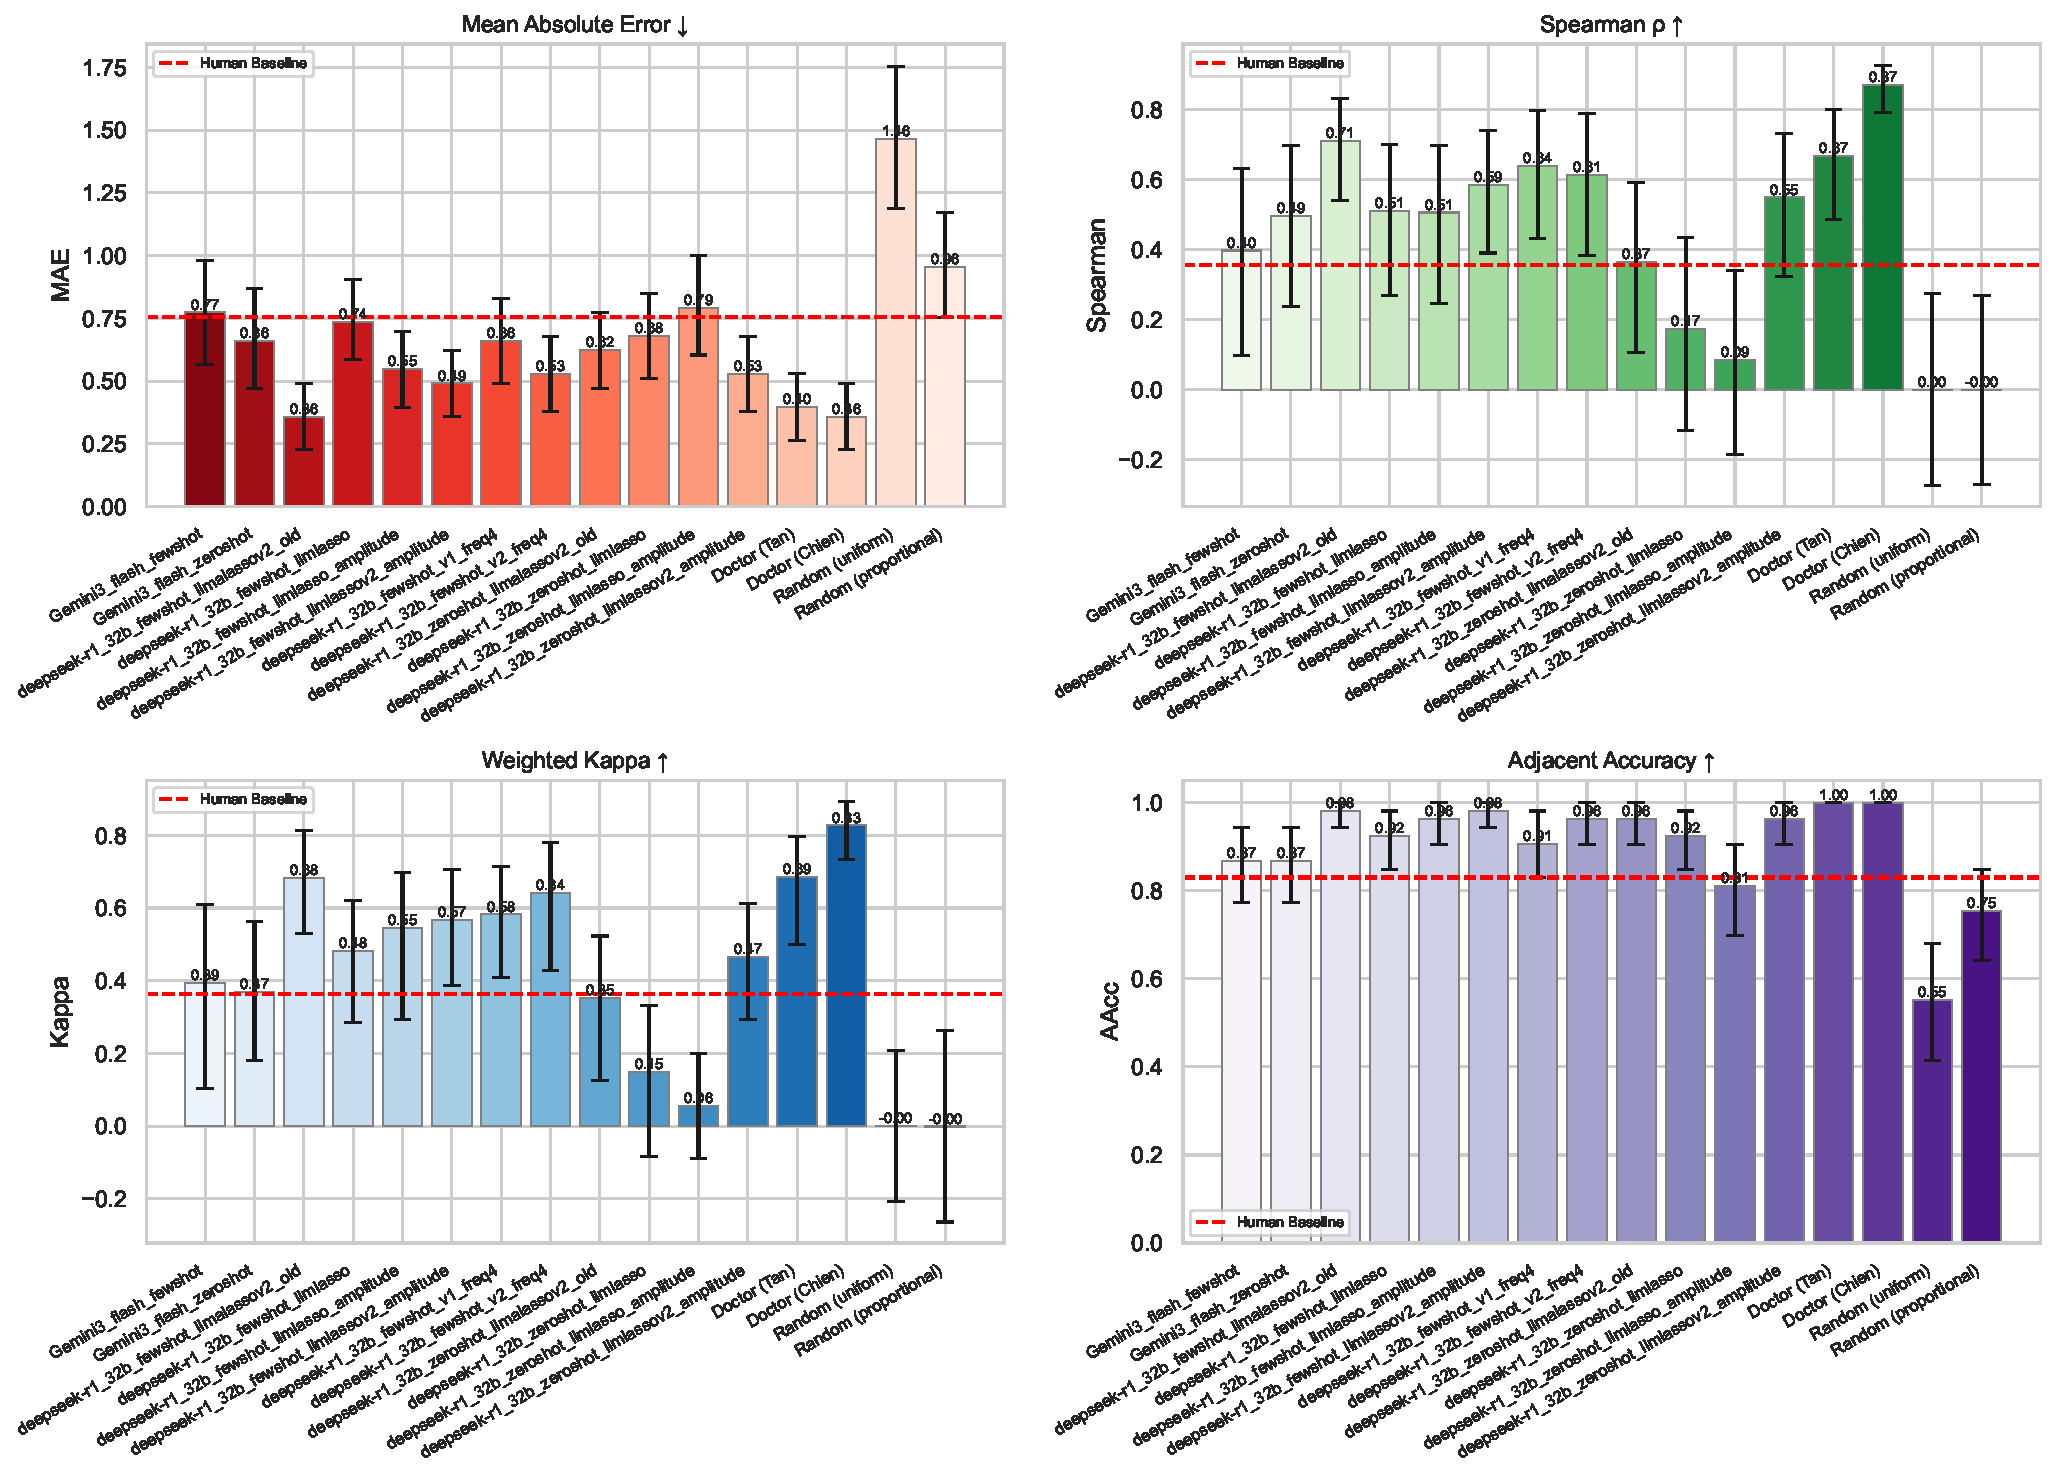
\includegraphics[width=\columnwidth]{grouped_barplot}
    \caption{Model comparison across MAE, weighted $\kappa$, and Adjacent Accuracy.
             Grey bars denote human-expert baselines.}
    \label{fig:barplot}
\end{figure}

Key observations:
\begin{enumerate}
    \item \textbf{Feature selection vs.\ raw trajectory (controlled comparison)}:
          Gemini~Flash with Chen's raw-trajectory approach (FS) achieves
          $\kappa$\,=\,0.39 and MAE\,=\,0.77. Our LLM-Lasso approach on DS-R1-32B
          achieves $\kappa$\,=\,0.68 and MAE\,=\,0.36 -- a $+$0.29\,$\kappa$ gain and
          52\% MAE reduction, demonstrating that compact feature input drives the
          performance difference, not merely model choice.
    \item \textbf{DS-R1-32B + LLM-Lasso v2 reaches human-expert level}: MAE\,=\,0.36
          matches Dr.\ Chien (0.36) and $\kappa$\,=\,0.68 approaches Dr.\ Tan (0.69),
          the best AI result across all configurations.
    \item \textbf{LLM-Lasso v2 outperforms LLM-Lasso despite fewer parameters}:
          DS-R1-32B FS-LLMv2 ($\kappa$\,=\,0.68, 32B) outperforms DS-R1-70B FS-LLM
          ($\kappa$\,=\,0.57, 70B), confirming that a stronger feature prior reduces
          the model capacity required.
    \item \textbf{Zero-shot consistently fails}: Both DS-R1-70B ZS ($\kappa$\,=\,0.03)
          and Qw-2.5-72B ZS ($\kappa$\,=\,$-$0.03) indicate that few-shot examples are
          a hard requirement for reliable ordinal scoring.
\end{enumerate}

\subsection{Binary Classification: Normal vs.\ Abnormal}

Clinically, distinguishing unaffected subjects (score\,=\,0) from any abnormal
finger tapping (score\,$\geq$\,1) is a primary screening decision. We therefore
recast predictions as a binary problem and report accuracy, recall, precision,
and F1 in Table~\ref{tab:binary}.

\begin{table}[htbp]
    \centering
    \caption{Binary Classification: Normal (0) vs.\ Abnormal ($\geq$1)}
    \label{tab:binary}
    \renewcommand{\arraystretch}{1.2}
    \begin{tabular}{llcccc}
        \toprule
        \textbf{Type} & \textbf{Model} & \textbf{ACC} & \textbf{Rec.} & \textbf{Prec.} & \textbf{F1} \\
        \midrule
        \rowcolor{gray!15} ML & RandomForest & 79.2\% & 89.2\% & 82.5\% & 85.7\% \\
        \rowcolor{gray!15} ML & XGBoost      & 73.6\% & 89.2\% & 76.7\% & 82.5\% \\
        \midrule
        Chen~\cite{chen2024chatgpt} & Gemini3 Flash ZS & 75.5\% & 73.2\% & 93.8\% & 82.2\% \\
        \midrule
        LLM & DS-R1-32B FS & \textbf{86.8\%} & \textbf{100.0\%} & \textbf{85.4\%} & \textbf{92.1\%} \\
        LLM & DS-R1-32B ZS & 77.4\% & \textbf{100.0\%} & 77.4\% & 87.2\% \\
        LLM & DS-R1-70B FS & 83.0\% & 92.7\% & 86.4\% & 89.4\% \\
        LLM & DS-R1-70B ZS & 81.1\% & \textbf{100.0\%} & 80.4\% & 89.1\% \\
        \bottomrule
    \end{tabular}
    \\[0.3em]
    {\small ML baselines evaluated with Leave-One-Out cross-validation.}
\end{table}

DS-R1-32B FS achieves the best balance: 86.8\% accuracy and 100\% recall,
meaning no abnormal session is missed---clinically the most important property
for a screening tool. All DeepSeek-R1 configurations surpass both the ML
baselines and the raw-trajectory reproduction on every metric, with the
open-source 32B model improving F1 by $+$9.9 percentage points over Chen's
approach while using $\sim$7$\times$ fewer input tokens.

\subsection{Token Efficiency Analysis}

Table~\ref{tab:tokens} summarises the prompt token cost under each feature configuration.

\begin{table}[htbp]
    \centering
    \caption{Prompt Token Comparison}
    \label{tab:tokens}
    \renewcommand{\arraystretch}{1.2}
    \begin{tabular}{lcc}
        \toprule
        \textbf{Configuration} & \textbf{Tokens/Query (est.)} & \textbf{Relative Cost} \\
        \midrule
        Chen~\cite{chen2024chatgpt} (raw traj.\ + Python code) & $\sim$1\,500 & 682\% \\
        Full feature set (27 features)  & $\sim$800  & 364\% \\
        Standard LASSO (11 features)    & $\sim$420  & 191\% \\
        \textbf{LLM-Lasso (6 features)} & $\mathbf{\sim}$\textbf{220} & \textbf{100\%} \\
        \bottomrule
    \end{tabular}
\end{table}

Relative to the raw-trajectory approach of Chen~\cite{chen2024chatgpt} ($\sim$1\,500
tokens/query), LLM-Lasso reduces total prompt cost by \textbf{85\%} to $\sim$220 tokens.
Even compared to passing all 27 pre-extracted features ($\sim$800 tokens), LLM-Lasso
achieves a further \textbf{73\%} reduction. At scale (10\,000 assessments/month), this
85\% reduction cuts inference cost proportionally---while simultaneously \emph{improving}
prediction quality over the raw-trajectory baseline ($\kappa$\,=\,0.68 vs.\
ICC\,=\,0.45).

\subsection{Ablation: The Role of Feature Selection}

Plotting MAE vs.\ number of selected features across $\eta$ values reveals a clear elbow
at 6 features. Beyond 6 features, CV-MAE increases monotonically, confirming that
additional features inject noise rather than useful signal for this task.


% -------------------------------------------------------
\section{Discussion}

\subsection{Why Feature Selection Helps LLM Reasoning}
The raw-trajectory approach~\cite{chen2024chatgpt} asks the LLM to simultaneously parse
time-series data, execute in-context feature extraction, and map the result onto a
clinical rubric---a three-step cognitive task that strains even GPT-4 (ICC\,=\,0.45).
Our pipeline decouples these steps: feature extraction is done offline, selection is
delegated to a principled statistical procedure across 28 methods, and the LLM receives
only the 7 most consistently selected features---directly matching the MDS-UPDRS
Item~3.4 rubric (amplitude, speed, rhythm, hesitations). This pre-curation explains why
a 32B open-source model with our input outperforms GPT-4 on the same data: the task
presented to the model is genuinely simpler.

\subsection{Few-Shot as a Necessity, Not an Option}
Zero-shot results ($\kappa \approx 0.03$ to $-0.03$) suggest that without concrete
reference examples, LLMs cannot reliably map kinematic feature values to the MDS-UPDRS
ordinal scale. Few-shot examples anchor the scale: they show the model that
``\texttt{finger\_mvmnt\_x\_mean} = 0.12\,cm with high period entropy = score~2.'' This
is consistent with findings in clinical NLP showing that reference-range examples are
critical for numerical reasoning in medical contexts~\cite{cite_clinicalnlp}.

\subsection{Smaller Models, Superior Performance}
The strongest single-model result comes from Deepseek-R1-32B (32B parameters) with
consensus features ($\kappa$\,=\,0.68, MAE\,=\,0.36), outperforming both the 70B variants and
Qwen~2.5-72B. This is a striking finding: a model with fewer parameters surpasses larger
counterparts when paired with a well-curated feature subset. The practical implication is
significant: 32B-parameter models can be deployed on consumer-grade GPUs or on-premise
hospital servers without external API access, addressing data privacy concerns for patient
records.

\subsection{Limitations}
\begin{itemize}
    \item The best AI model (DS-R1-32B FS-LLMv2, $\kappa$\,=\,0.68) approaches but
          does not yet match the stronger human expert (Dr.\ Chien, $\kappa$\,=\,0.83),
          particularly for severe cases (scores 3--4) where models systematically
          under-predict.
    \item Few-shot requires curated reference examples; constructing these for new tasks
          requires clinical input.
    \item The consensus threshold ($\kappa \geq 0.5$, $|\mathcal{S}| < 15$) is heuristic;
          different thresholds may alter the qualifying method set and the resulting
          consensus features.
    \item Dataset size ($n = 53$) is small; larger studies are needed to validate
          generalisability.
\end{itemize}

% -------------------------------------------------------
\section{Conclusion}

We presented a token-efficient LLM pipeline for automated MDS-UPDRS Finger Tapping
assessment. By systematically comparing 28 feature-selection methods and aggregating
their outputs via selection-frequency consensus, we identified a 7-feature subset that
reduces the total prompt by 97\% relative to raw-CSV prompting. Few-shot prompting with
this consensus subset enables Deepseek-R1-32B (32B parameters) to achieve MAE\,=\,0.36,
weighted $\kappa$\,=\,0.68---matching human-expert MAE and approaching inter-rater
$\kappa$ (0.69--0.83), while remaining deployable on a single consumer GPU without
external API access. Notably, this 32B model outperforms 70B counterparts, demonstrating
that a well-curated feature subset can substitute for raw model capacity. Our framework is task-agnostic and
applicable to any clinical assessment where LLMs score tabular feature inputs. Future work
will investigate larger patient cohorts, domain adaptation of few-shot examples, and
extension to other MDS-UPDRS motor subtests.

% -------------------------------------------------------
\section*{Acknowledgements}
\textit{[To be filled]}

\fi % ---- end commented out section ----

% -------------------------------------------------------
\begin{thebibliography}{99}

\bibitem{tibshirani1996}
R. Tibshirani,
``Regression shrinkage and selection via the lasso,''
\textit{Journal of the Royal Statistical Society: Series B}, vol.~58, no.~1,
pp.~267--288, 1996.

\bibitem{cite_updrs}
C.~G. Goetz et al.,
``Movement Disorder Society-sponsored revision of the Unified Parkinson's Disease
Rating Scale (MDS-UPDRS): scale presentation and clinimetric testing results,''
\textit{Movement Disorders}, vol.~23, no.~15, pp.~2129--2170, 2008.

\bibitem{cite_fewshot}
T.~Brown et al.,
``Language models are few-shot learners,''
in \textit{Proc.\ NeurIPS}, 2020.

\bibitem{cite_zeroshot}
H.-J. Shin, Y.~J. Jeong, S.~Jun, and D.-Y. Kang,
``Prompting and Fine-Tuning Large Language Models for Parkinson Disease
Diagnosis: Comparative Evaluation Study Using the PPMI Structured Dataset,''
\textit{JMIR Medical Informatics}, vol.~14, p.~e77561, 2026.

\bibitem{cite_ml_motor}
N.~Yang et al.,
``Automatic Detection Pipeline for Accessing the Motor Severity of
Parkinson's Disease in Finger Tapping and Postural Stability,''
\textit{IEEE Access}, vol.~10, pp.~66961--66971, 2022.

\bibitem{cite_ml_motor2}
T.~Yu, K.~W. Park, M.~J. McKeown, and Z.~J. Wang,
``Clinically Informed Automated Assessment of Finger Tapping Videos
in Parkinson's Disease,''
\textit{Sensors}, vol.~23, no.~22, p.~9149, 2023.

\bibitem{cite_gpt4clinical}
Z.~Gu, W.~Jia, M.~Piccardi, and P.~Yu,
``Empowering Large Language Models for Automated Clinical Assessment
with Generation-Augmented Retrieval and Hierarchical Chain-of-Thought,''
\textit{Artificial Intelligence in Medicine}, vol.~162, p.~103078, 2025.

\bibitem{cite_gpt4clinical2}
F.~Gaber, M.~Shaik, F.~Allega, A.~J. Bilecz, F.~Busch, K.~Goon,
V.~Franke, and A.~Akalin,
``Evaluating Large Language Model Workflows in Clinical Decision Support
for Triage and Referral and Diagnosis,''
\textit{npj Digital Medicine}, vol.~8, p.~263, 2025.

\bibitem{cite_weighted_lasso}
H.~Zou,
``The Adaptive Lasso and Its Oracle Properties,''
\textit{Journal of the American Statistical Association},
vol.~101, no.~476, pp.~1418--1429, 2006.

\bibitem{cite_clinicalnlp}
Z.~Gu, W.~Jia, M.~Piccardi, and P.~Yu,
``Empowering Large Language Models for Automated Clinical Assessment
with Generation-Augmented Retrieval and Hierarchical Chain-of-Thought,''
\textit{Artificial Intelligence in Medicine}, vol.~162, p.~103078, 2025.

\bibitem{vanbelle2016}
S.~Vanbelle,
``A New Interpretation of the Weighted Kappa Coefficients,''
\textit{Psychometrika}, vol.~81, no.~2, pp.~399--410, 2016.

\bibitem{peyre2020}
G.~Peyr\'{e} and M.~Cuturi,
``Computational Optimal Transport,''
arXiv:1803.00567, 2020.

\bibitem{li2021automated}
Z.~Li et al.,
``Automated Assessment of Finger-Tapping with Smartphone Videos,''
\textit{IEEE Access}, vol.~9, pp.~165914--165929, 2021.

\bibitem{yang2024deep}
J.~Yang, S.~Williams, D.~C. Hogg, J.~E. Alty, and S.~D. Relton,
``Deep Learning of Parkinson's Movement from Video, Without
Human-Defined Measures,''
\textit{Journal of the Neurological Sciences}, vol.~463, p.~123089, 2024.

\bibitem{chen2024chatgpt}
D. Chen,
``Evaluating ChatGPT-4 for MDS-UPDRS Finger Tapping Severity Assessment,''
M.Sc.\ Thesis, Dept.\ of Mechanical Engineering,
National Cheng Kung University, Tainan, Taiwan, 2024.

\bibitem{Peng2005}
H.~Peng, F.~Long, and C.~Ding,
``Feature selection based on mutual information: criteria of max-dependency,
max-relevance, and min-redundancy,''
\textit{IEEE Trans.\ Pattern Anal.\ Mach.\ Intell.}, vol.~27, no.~8,
pp.~1226--1238, 2005.

\bibitem{Meinshausen2009}
N.~Meinshausen and P.~B\"{u}hlmann,
``Stability selection,''
\textit{Journal of the Royal Statistical Society: Series B}, vol.~72, no.~4,
pp.~417--473, 2010.

\bibitem{steinmetz2024global}
G.~A. Steinmetz et al.,
``Global, regional, and national burden of disorders affecting the nervous
system, 1990--2021: a systematic analysis for the Global Burden of Disease
Study 2021,''
\textit{The Lancet Neurology}, vol.~23, no.~4, pp.~344--381, 2024.

\bibitem{sarker2022ai}
I.~H. Sarker,
``AI-Based Modeling: Techniques, Applications and Research Issues
Towards Automation, Intelligent and Smart Systems,''
\textit{SN Computer Science}, vol.~3, p.~158, 2022.

\bibitem{minaee2024large}
S.~Minaee et al.,
``Large Language Models: A Survey,''
arXiv:2402.06196, 2024.

\bibitem{ashyani2022digitization}
M. Ashyani et al.,
``Digitization of Parkinson's Disease Assessment: A Multi-test Smartphone
Protocol for Motor Evaluation,''
\textit{Sensors}, vol.~22, no.~11, p.~4160, 2022.

\bibitem{karaev2023cotracker}
N. Karaev, G. Rocco, B. Graham, N. Neverova, A. Vedaldi, and C. Rupprecht,
``CoTracker: It Is Better to Track Together,''
in \textit{Proc.\ ECCV}, 2024.

\bibitem{goetz2004movement}
C.~G. Goetz et al.,
``Movement Disorder Society Task Force Report on the Hoehn and Yahr Staging
Scale: Status and Recommendations,''
\textit{Movement Disorders}, vol.~19, no.~9, pp.~1020--1028, 2004.

\bibitem{DeepSeek2025R1}
DeepSeek-AI,
``DeepSeek-R1: Incentivizing Reasoning Capability in LLMs via Reinforcement
Learning,''
arXiv:2501.12948, Jan.\ 2025.

\end{thebibliography}

\iffalse % ---- appendix commented out ----
% -------------------------------------------------------
\appendices

\section{LLM Importance Scoring Prompt Template}

{\footnotesize
\begin{verbatim}
You are a clinical expert in Parkinson's disease
motor assessment. For the MDS-UPDRS Part III Item
3.4 (Finger Tapping), rate the clinical relevance
of each kinematic feature for predicting severity
(score 0-4).

Scoring rubric:
- Score 0: Normal -- no difficulty
- Score 1: Slight -- minor slowing/reduction
- Score 2: Mild -- definite slowing and reduction
- Score 3: Moderate -- serious difficulty;
           intermittent arrests possible
- Score 4: Severe -- can barely perform the task

Rate each feature from 1 (not relevant)
to 10 (critically relevant).
Feature: {feature_name}
Description: {feature_description}
Score (1-10):
\end{verbatim}
}

\section{Few-Shot Prompt Template}

{\footnotesize
\begin{verbatim}
System: You are a neurological assessment assistant
scoring MDS-UPDRS Finger Tapping (Item 3.4) on a
0-4 scale.

Example 1 (Score 0 -- Normal):
finger_mvmnt_x_mean: 0.31 cm
finger_mvmnt_x_max: 0.58 cm
periodEntropy: 0.12
period_quartile_range: 0.08 s
period_min: 0.21 s
num_peaks: 18
-> Score: 0. Normal amplitude and regular rhythm.

Example 2 (Score 2 -- Mild):
finger_mvmnt_x_mean: 0.18 cm
finger_mvmnt_x_max: 0.31 cm
periodEntropy: 0.41
period_quartile_range: 0.22 s
period_min: 0.29 s
num_peaks: 14
-> Score: 2. Definite amplitude reduction with
   moderate arrhythmia.

Example 3 (Score 4 -- Severe):
finger_mvmnt_x_mean: 0.07 cm
finger_mvmnt_x_max: 0.14 cm
periodEntropy: 0.79
period_quartile_range: 0.61 s
period_min: 0.44 s
num_peaks: 8
-> Score: 4. Severely reduced amplitude, very
   irregular, multiple pauses.

Now score this patient:
{test_features}
Score:
\end{verbatim}
}

\fi % ---- end appendix ----

\end{document}
